\section{Aplicación}\label{Application}

\begin{figure}[H]
	\centering
	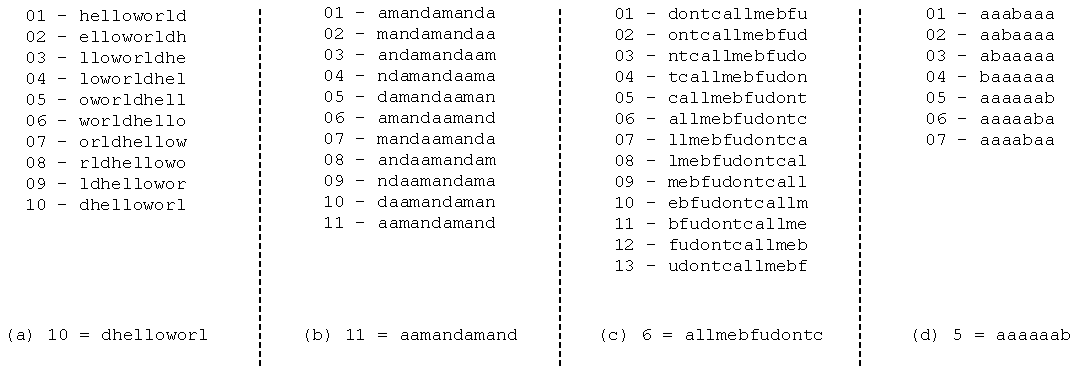
\includegraphics[width=0.8\linewidth]{doc/Application/img/cases-necklace}
	\caption{Problema: \textit{UVA 719 - Glass Beads}. Casos de entrada que contienen la descripción del collar y el número de la perla que es la primera en la peor separación posible. Cada perla está representada por un carácter en minúscula del alfabeto inglés $(a–z)$, donde $a < b < ... < z$. (a) $helloworld$. (b) $amandamanda$. (c) $dontcallmebfu$. (d) $aaabaaa$. }
	\label{fig:UVA-719-Input-Output}
\end{figure}


\renewcommand{\lstlistingname}{Implementación}% Listing -> Algorithm
\renewcommand{\lstlistlistingname}{Lista de \lstlistingname s}% List of Listings -> List of Algorithms
\lstset{
	tabsize=2,% tab space width
	basicstyle=\scriptsize,
	showstringspaces=false, % don't mark spaces in strings
	numbers=left, % display line numbers on the left
	numbersep=\intextsep,
	commentstyle=\color{green}, % comment color
	keywordstyle=\color{blue}, % keyword color
	stringstyle=\color{red}, % string color
	xleftmargin=\marginparsep
}
\lstinputlisting[label=SuffixAutomaton, caption=Caption, language=C++]{doc/Application/code/GlassBeads.cpp}